\documentclass[11pt]{beamer}
\usetheme{PaloAlto}
\usepackage[utf8]{inputenc}
\usepackage{amsmath}
\usepackage{amsfonts}
\usepackage{amssymb}
\usepackage{graphicx}
\author{NANDAKISHOR S\\RANJITH R\\MOHAMMED AFRIDI}
\title{SLAYTER\\	( GAME USING PYTHON  GRAPHICS)}
%\setbeamercovered{transparent} 
%\setbeamertemplate{navigation symbols}{} 
%\logo{} 
%\institute{} 
%\date{} 
%\subject{} 
\begin{document}

\begin{frame}
\titlepage
\end{frame}

%\begin{frame}
%\tableofcontents
%\end{frame}

\begin{frame}{INTRODUCTION}
\begin{itemize}
\item The objective is to create a 2-D vedio game using python programming language.
\item The existing 2-d games lack user friendly interface, most of them have text based interface.
\item In order to solve this problem and give the user a better gaming experience we are creating this game namely "SLAYTER"

\end{itemize}

\end{frame}

\begin{frame}{OBJECTIVE}
\begin{itemize}
\item THE OBJECTIVE OF THE GAME IS TO KILL AS MANY DEMONS AS POSSIBLE AND COLLECTS POINTS AND COINS IN ORDER TO ADVANCE TO HIGHER LEVELS

 
\item STORY LINE : \\
The aim of the game is to defend our home village.

The village has been attacked by demons quite frequently.

The village has no one left to fight as the demons have already killed the ones willing to fight.

And finally it is our job to be the defender of our village,\\THE LAST HOPE 

\end{itemize}

\end{frame}

\begin{frame}{PROPOSED SYSTEM and ITS BLOCK DIAGRAM}
\begin{itemize}
\item The game is created in python programming language.
\item The game interface is very simple and logical with toolbars and creative and intuitive controls designed for a better gaming experience.
\end{itemize}
\end{frame}

\begin{frame}
\begin{center}
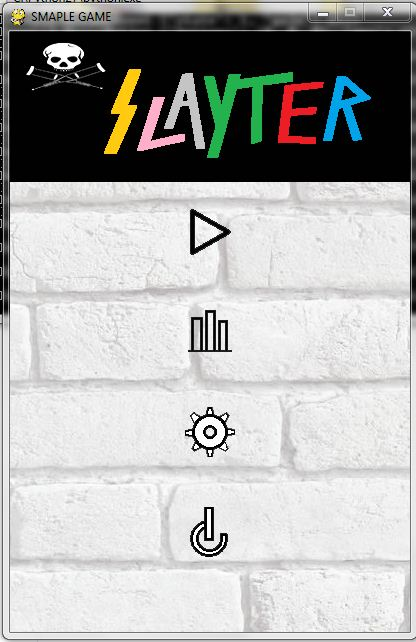
\includegraphics[scale=0.5]{Capture.jpg}
\end{center}
\end{frame}


\begin{frame}{SOFTWARE AND HARDWARE REQUIREMENTS}
\begin{itemize}
\item SOFTWARE REQUIREMENTS
\begin{itemize}
\item OS: Windows xp or above / UBUNTU 13+ / LINUX  
\item PYTHON INTERPRETER OR SHELL
\item PYGAME MODULE HAS TO BE INSTALLED
\item ADOBE PHOTOSHOP CS 3(OR ABOVE)
\item MS PAINT
\end{itemize}
\item HARDWARE REQUIREMENTS
\begin{itemize}
\item RAM : 1GB+
\item MIN MEMORY AVAILABLE: 10 MB
\item MIN INBUILT GRAPHICS REQUIRED
\item SPEAKERS, MONITOR, KEYBOARD AND MOUSE
\end{itemize}
\end{itemize}
\end{frame}

\begin{frame}{ALGORITHM}
STEPS : \\
\begin{enumerate}
\item START
\item THE GAME LOOP STARTS AND ALL THE PARAMETERS GET INITIALISED ALONG WITH PYGAME
\item THE START PAGE IS PRINTED ON THE SCREEN OF \\DIMENSIONS 400 X 600
\item THE START SCREEN CONTAINS 4 OPTIONS(BUTTONS)
\begin{itemize}
\item PLAY
\item STATISTICS
\item SETTINGS
\item QUIT OPTION : ALLOWS TO QUIT THE GAME
\item PLAY IS RUN ON ANOTHER PROGRAM WHICH WILL BE IMPORTED 
\item AFTER CONVERTING THE THE GAME IT CAN BE EASILY EQUALISED
\end{itemize}
\end{enumerate}
\end{frame}



\begin{frame}{MODULES}
\begin{itemize}
\item pygame module
\item random
\item time\\
\end{itemize}

\end{frame}


 
\begin{frame}{CONCLUSION}
The game after preparation would be very attracive and user friendly

\end{frame}
\end{document}
